\documentclass{standalone}
\usepackage{tikz}
\usetikzlibrary{patterns, positioning}


\begin{document}
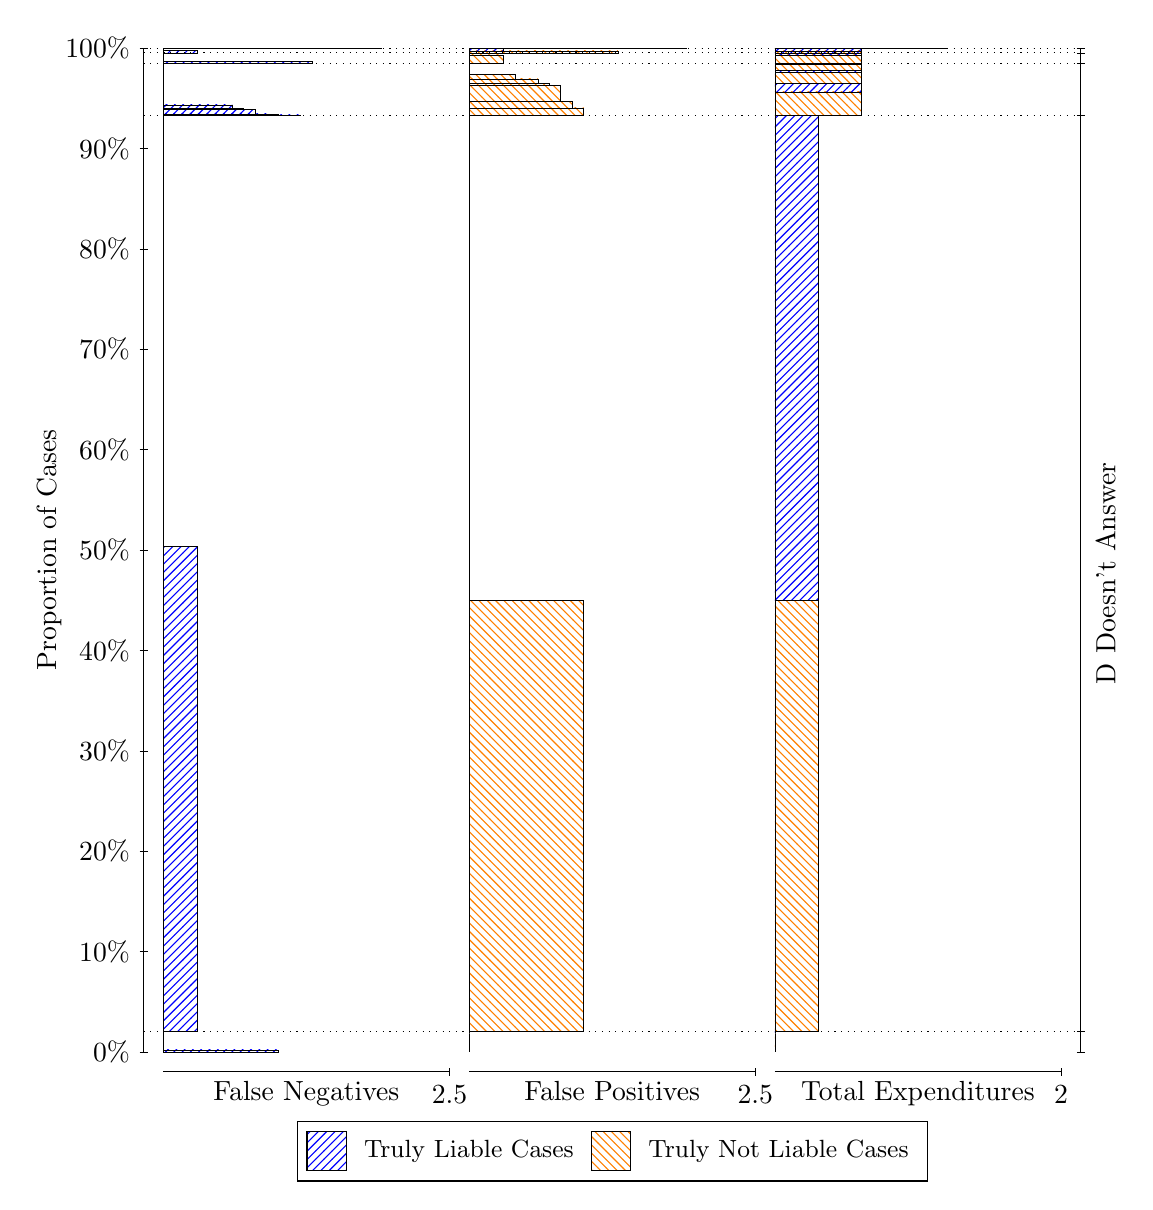
\begin{tikzpicture}
\draw[black, very thin] (1.5,1.75) -- (1.5,14.5);
\node[rotate=90, text=black, anchor=center] at (0.3, 8.125) {Proportion of Cases};
\draw[black, very thin] (1.45,1.75) -- (1.55,1.75);
\node[text=black, anchor=east] at (1.45, 1.75) {0\%};
\draw[black, very thin] (1.45,3.025) -- (1.55,3.025);
\node[text=black, anchor=east] at (1.45, 3.025) {10\%};
\draw[black, very thin] (1.45,4.3) -- (1.55,4.3);
\node[text=black, anchor=east] at (1.45, 4.3) {20\%};
\draw[black, very thin] (1.45,5.575) -- (1.55,5.575);
\node[text=black, anchor=east] at (1.45, 5.575) {30\%};
\draw[black, very thin] (1.45,6.85) -- (1.55,6.85);
\node[text=black, anchor=east] at (1.45, 6.85) {40\%};
\draw[black, very thin] (1.45,8.125) -- (1.55,8.125);
\node[text=black, anchor=east] at (1.45, 8.125) {50\%};
\draw[black, very thin] (1.45,9.4) -- (1.55,9.4);
\node[text=black, anchor=east] at (1.45, 9.4) {60\%};
\draw[black, very thin] (1.45,10.675) -- (1.55,10.675);
\node[text=black, anchor=east] at (1.45, 10.675) {70\%};
\draw[black, very thin] (1.45,11.95) -- (1.55,11.95);
\node[text=black, anchor=east] at (1.45, 11.95) {80\%};
\draw[black, very thin] (1.45,13.225) -- (1.55,13.225);
\node[text=black, anchor=east] at (1.45, 13.225) {90\%};
\draw[black, very thin] (1.45,14.5) -- (1.55,14.5);
\node[text=black, anchor=east] at (1.45, 14.5) {100\%};

\draw[black, very thin] (13.4,1.75) -- (13.4,14.5);
\draw[black, very thin] (13.35,1.75) -- (13.45,1.75);
\node[anchor=west] at (13.35, 1.75) {};
\draw[black, very thin] (13.35,2.0136) -- (13.45,2.0136);
\node[anchor=west] at (13.35, 2.0136) {};
\draw[black, very thin] (13.35,13.643) -- (13.45,13.643);
\node[anchor=west] at (13.35, 13.643) {};
\draw[black, very thin] (13.35,14.302) -- (13.45,14.302);
\node[anchor=west] at (13.35, 14.302) {};
\draw[black, very thin] (13.35,14.439) -- (13.45,14.439);
\node[anchor=west] at (13.35, 14.439) {};
\draw[black, very thin] (13.35,14.494) -- (13.45,14.494);
\node[anchor=west] at (13.35, 14.494) {};
\draw[black, very thin] (13.35,14.497) -- (13.45,14.497);
\node[anchor=west] at (13.35, 14.497) {};
\draw[black, very thin] (13.35,14.5) -- (13.45,14.5);
\node[anchor=west] at (13.35, 14.5) {};

\draw[black, very thin, pattern color=blue, pattern=north east lines] (1.75,1.75) rectangle (3.2033,1.7777);
\draw[black, very thin, pattern color=orange, pattern=north west lines] (1.75,1.7777) rectangle (1.75,2.0136);
\draw[black, very thin, pattern color=blue, pattern=north east lines] (1.75,2.0136) rectangle (2.186,8.1682);
\draw[black, very thin, pattern color=orange, pattern=north west lines] (1.75,8.1682) rectangle (1.75,13.643);
\draw[black, very thin, pattern color=blue, pattern=north east lines] (1.75,13.643) rectangle (3.494,13.651);
\draw[black, very thin, pattern color=blue, pattern=north east lines] (1.75,13.651) rectangle (3.2033,13.656);
\draw[black, very thin, pattern color=blue, pattern=north east lines] (1.75,13.656) rectangle (3.058,13.664);
\draw[black, very thin, pattern color=blue, pattern=north east lines] (1.75,13.664) rectangle (2.9127,13.725);
\draw[black, very thin, pattern color=blue, pattern=north east lines] (1.75,13.725) rectangle (2.7673,13.735);
\draw[black, very thin, pattern color=blue, pattern=north east lines] (1.75,13.735) rectangle (2.622,13.777);
\draw[black, very thin, pattern color=orange, pattern=north west lines] (1.75,13.777) rectangle (1.75,14.302);
\draw[black, very thin, pattern color=blue, pattern=north east lines] (1.75,14.302) rectangle (3.6393,14.328);
\draw[black, very thin, pattern color=orange, pattern=north west lines] (1.75,14.328) rectangle (1.75,14.439);
\draw[black, very thin, pattern color=blue, pattern=north east lines] (1.75,14.439) rectangle (2.186,14.47);
\draw[black, very thin, pattern color=orange, pattern=north west lines] (1.75,14.47) rectangle (1.75,14.494);
\draw[black, very thin, pattern color=blue, pattern=north east lines] (1.75,14.494) rectangle (4.5113,14.495);
\draw[black, very thin, pattern color=orange, pattern=north west lines] (1.75,14.495) rectangle (1.75,14.497);
\draw[black, very thin, pattern color=blue, pattern=north east lines] (1.75,14.497) rectangle (2.186,14.499);
\draw[black, very thin, pattern color=orange, pattern=north west lines] (1.75,14.499) rectangle (1.75,14.5);
\draw[black, very thin, pattern color=orange, pattern=north west lines] (5.6333,1.75) rectangle (5.6333,1.9859);
\draw[black, very thin, pattern color=blue, pattern=north east lines] (5.6333,1.9859) rectangle (5.6333,2.0136);
\draw[black, very thin, pattern color=orange, pattern=north west lines] (5.6333,2.0136) rectangle (7.0867,7.4883);
\draw[black, very thin, pattern color=blue, pattern=north east lines] (5.6333,7.4883) rectangle (5.6333,13.643);
\draw[black, very thin, pattern color=orange, pattern=north west lines] (5.6333,13.643) rectangle (7.0867,13.741);
\draw[black, very thin, pattern color=orange, pattern=north west lines] (5.6333,13.741) rectangle (6.9413,13.819);
\draw[black, very thin, pattern color=orange, pattern=north west lines] (5.6333,13.819) rectangle (6.796,14.022);
\draw[black, very thin, pattern color=orange, pattern=north west lines] (5.6333,14.022) rectangle (6.6507,14.053);
\draw[black, very thin, pattern color=orange, pattern=north west lines] (5.6333,14.053) rectangle (6.5053,14.108);
\draw[black, very thin, pattern color=orange, pattern=north west lines] (5.6333,14.108) rectangle (6.2147,14.168);
\draw[black, very thin, pattern color=blue, pattern=north east lines] (5.6333,14.168) rectangle (5.6333,14.302);
\draw[black, very thin, pattern color=orange, pattern=north west lines] (5.6333,14.302) rectangle (6.0693,14.414);
\draw[black, very thin, pattern color=blue, pattern=north east lines] (5.6333,14.414) rectangle (5.6333,14.439);
\draw[black, very thin, pattern color=orange, pattern=north west lines] (5.6333,14.439) rectangle (7.5227,14.463);
\draw[black, very thin, pattern color=blue, pattern=north east lines] (5.6333,14.463) rectangle (6.0693,14.494);
\draw[black, very thin, pattern color=orange, pattern=north west lines] (5.6333,14.494) rectangle (6.0693,14.496);
\draw[black, very thin, pattern color=blue, pattern=north east lines] (5.6333,14.496) rectangle (5.6333,14.497);
\draw[black, very thin, pattern color=orange, pattern=north west lines] (5.6333,14.497) rectangle (8.3947,14.498);
\draw[black, very thin, pattern color=blue, pattern=north east lines] (5.6333,14.498) rectangle (6.9413,14.5);
\draw[black, very thin, pattern color=orange, pattern=north west lines] (9.5167,1.75) rectangle (9.5167,1.9859);
\draw[black, very thin, pattern color=blue, pattern=north east lines] (9.5167,1.9859) rectangle (9.5167,2.0136);
\draw[black, very thin, pattern color=orange, pattern=north west lines] (9.5167,2.0136) rectangle (10.062,7.4883);
\draw[black, very thin, pattern color=blue, pattern=north east lines] (9.5167,7.4883) rectangle (10.062,13.643);
\draw[black, very thin, pattern color=orange, pattern=north west lines] (9.5167,13.643) rectangle (10.607,13.943);
\draw[black, very thin, pattern color=blue, pattern=north east lines] (9.5167,13.943) rectangle (10.607,14.046);
\draw[black, very thin, pattern color=orange, pattern=north west lines] (9.5167,14.046) rectangle (10.607,14.193);
\draw[black, very thin, pattern color=blue, pattern=north east lines] (9.5167,14.193) rectangle (10.607,14.214);
\draw[black, very thin, pattern color=orange, pattern=north west lines] (9.5167,14.214) rectangle (10.607,14.293);
\draw[black, very thin, pattern color=blue, pattern=north east lines] (9.5167,14.293) rectangle (10.607,14.302);
\draw[black, very thin, pattern color=orange, pattern=north west lines] (9.5167,14.302) rectangle (10.607,14.414);
\draw[black, very thin, pattern color=blue, pattern=north east lines] (9.5167,14.414) rectangle (10.607,14.439);
\draw[black, very thin, pattern color=orange, pattern=north west lines] (9.5167,14.439) rectangle (10.607,14.463);
\draw[black, very thin, pattern color=blue, pattern=north east lines] (9.5167,14.463) rectangle (10.607,14.494);
\draw[black, very thin, pattern color=orange, pattern=north west lines] (9.5167,14.494) rectangle (11.697,14.496);
\draw[black, very thin, pattern color=blue, pattern=north east lines] (9.5167,14.496) rectangle (11.697,14.497);
\draw[black, very thin, pattern color=orange, pattern=north west lines] (9.5167,14.497) rectangle (11.697,14.498);
\draw[black, very thin, pattern color=blue, pattern=north east lines] (9.5167,14.498) rectangle (11.697,14.5);
\draw[black, dotted] (1.5,2.0136) -- (13.4,2.0136);
\draw[black, dotted] (1.5,13.643) -- (13.4,13.643);
\draw[black, dotted] (1.5,14.302) -- (13.4,14.302);
\draw[black, dotted] (1.5,14.439) -- (13.4,14.439);
\draw[black, dotted] (1.5,14.494) -- (13.4,14.494);
\draw[black, dotted] (1.5,14.497) -- (13.4,14.497);
\draw[black, very thin] (1.75,1.5) -- (5.3833,1.5);
\node[text=black, anchor=north] at (3.5667, 1.5) {False Negatives};
\draw[black, very thin] (5.3833,1.45) -- (5.3833,1.55);
\node[text=black, anchor=north] at (5.3833, 1.45) {2.5};

\draw[black, very thin] (5.6333,1.5) -- (9.2667,1.5);
\node[text=black, anchor=north] at (7.45, 1.5) {False Positives};
\draw[black, very thin] (9.2667,1.45) -- (9.2667,1.55);
\node[text=black, anchor=north] at (9.2667, 1.45) {2.5};

\draw[black, very thin] (9.5167,1.5) -- (13.15,1.5);
\node[text=black, anchor=north] at (11.333, 1.5) {Total Expenditures};
\draw[black, very thin] (13.15,1.45) -- (13.15,1.55);
\node[text=black, anchor=north] at (13.15, 1.45) {2};


\node[text=black, centered, rotate=90] at (13.72, 7.8283) {D Doesn't Answer};






\draw (7.449999999999999,1.5) node[draw=none] (baseCoordinate) {};
\begin{scope}[align=center]
        \matrix[scale=0.5, draw=black, below=0.5cm of baseCoordinate, nodes={draw}, column sep=0.1cm]{
            \node[rectangle, draw, minimum width=0.5cm, minimum height=0.5cm, pattern color=blue, pattern=north east lines] {}; &
            \node[draw=none, font=\small, text=black] (B) {Truly Liable Cases}; &
            \node[rectangle, draw, minimum width=0.5cm, minimum height=0.5cm, pattern color=orange, pattern=north west lines] {}; &
            \node[draw=none, font=\small, text=black] (B) {Truly Not Liable Cases}; \\
            };
\end{scope}

\end{tikzpicture}
\end{document}